\begin{solution}{normal}
\textbf{(a)} \begin{proof} We note that the total change in energy is given by
\begin{align*}
\Delta U &= n C_V\Delta T\\
&= C_Vn_1(T - T_1) + C_Vn_2(T - T_2)
\end{align*}By the ideal gas law, $pV = n RT$, we have that
\[\Delta U = \frac{C_Vp_0(V - V_1 - V_2)}{R}\]we also see that internal energy change must be equal to the work produced by external pressure. Therefore,
\[\frac{C_Vp_0(V - V_1 - V_2)}{R} = p_0 (V - V_1 - V_2).\]Since $C_V/R$ is non-zero we find that
\[V- V_1 - V_2 = 0\implies V = V_1 + V_2.\]
\end{proof}
\vspace{3mm}

\noindent \textbf{(b)} We note that by the ideal gas law
\[pV = n RT\implies n = \frac{pV}{RT}.\]This tells us that the moles of gas in our scenario is given as
\[n = \frac{p_0}{R}\left(\frac{V_1}{T_1} + \frac{V_2}{T_2}\right) = \frac{p_0}{R}\left(\frac{V_1 + V_2}{T^{\prime}}\right)\]therefore, we find that
\[T^{\prime} = \frac{V_1 + V_2}{V_1/T_1 + V_2/T_2}\approx \boxed{16.5^{\circ}\;\mathrm{C}}\]
\vspace{3mm}

\noindent \textbf{(c)} Note that relative humidity is denoted as the mass of water vapor divided by the mass of water vapor in saturation. In this problem, we have to calculate the relative humidity of the mixed air. First, note that y-axis of the graph that is given in part (c) represents density. We have to convert our mass relation to density which is fairly easy as the density is directly proportional to mass which means that $r = \frac{\rho_v}{\rho_{\text{vs}}}$.
\vspace{3mm}

\noindent Next, we need to determine these two densities. First, note that there were two individual mixtures of air, one, inside the room at temperature $t_1 = 25^{\circ}\;\mathrm{C}$ and the other outside of the room at temperature $t_2 = 1^{\circ}\;\mathrm{C}$. We mark these two points on our graph as point 1 and 2 respectively. We then connect these two points with a line. The temperature of the mixed air as shown in part (b) is $16.5^{\circ}\;\mathrm{C}$. The density of the water vapor while be the intersection of the line $x = 16.5$ and the line connecting the two points 1 and 2. By finding the intersection of these two points, we find that $\rho_v$ is at point 3 with a density of $1.65\;\mathrm{g/m^3}$. The mass of the water vapor in saturation is represented by the intersection of the graph and the line $x = 16.5$ (this is because the graph shows the dependence of saturated vapor density of water as a function of temperature). This gives us the point 4 with a density of $\rho_{\text{vs}} = 1.37\;\mathrm{g/cm^3}$. We now finally obtain the relative humidity to be
\[r = \frac{\rho_v}{\rho_{\text{vs}}} = \frac{1.65\;\mathrm{g/cm^3}}{1.37\;\mathrm{g/cm^3}} = 1.20 = 120\%.\]
\begin{center}
    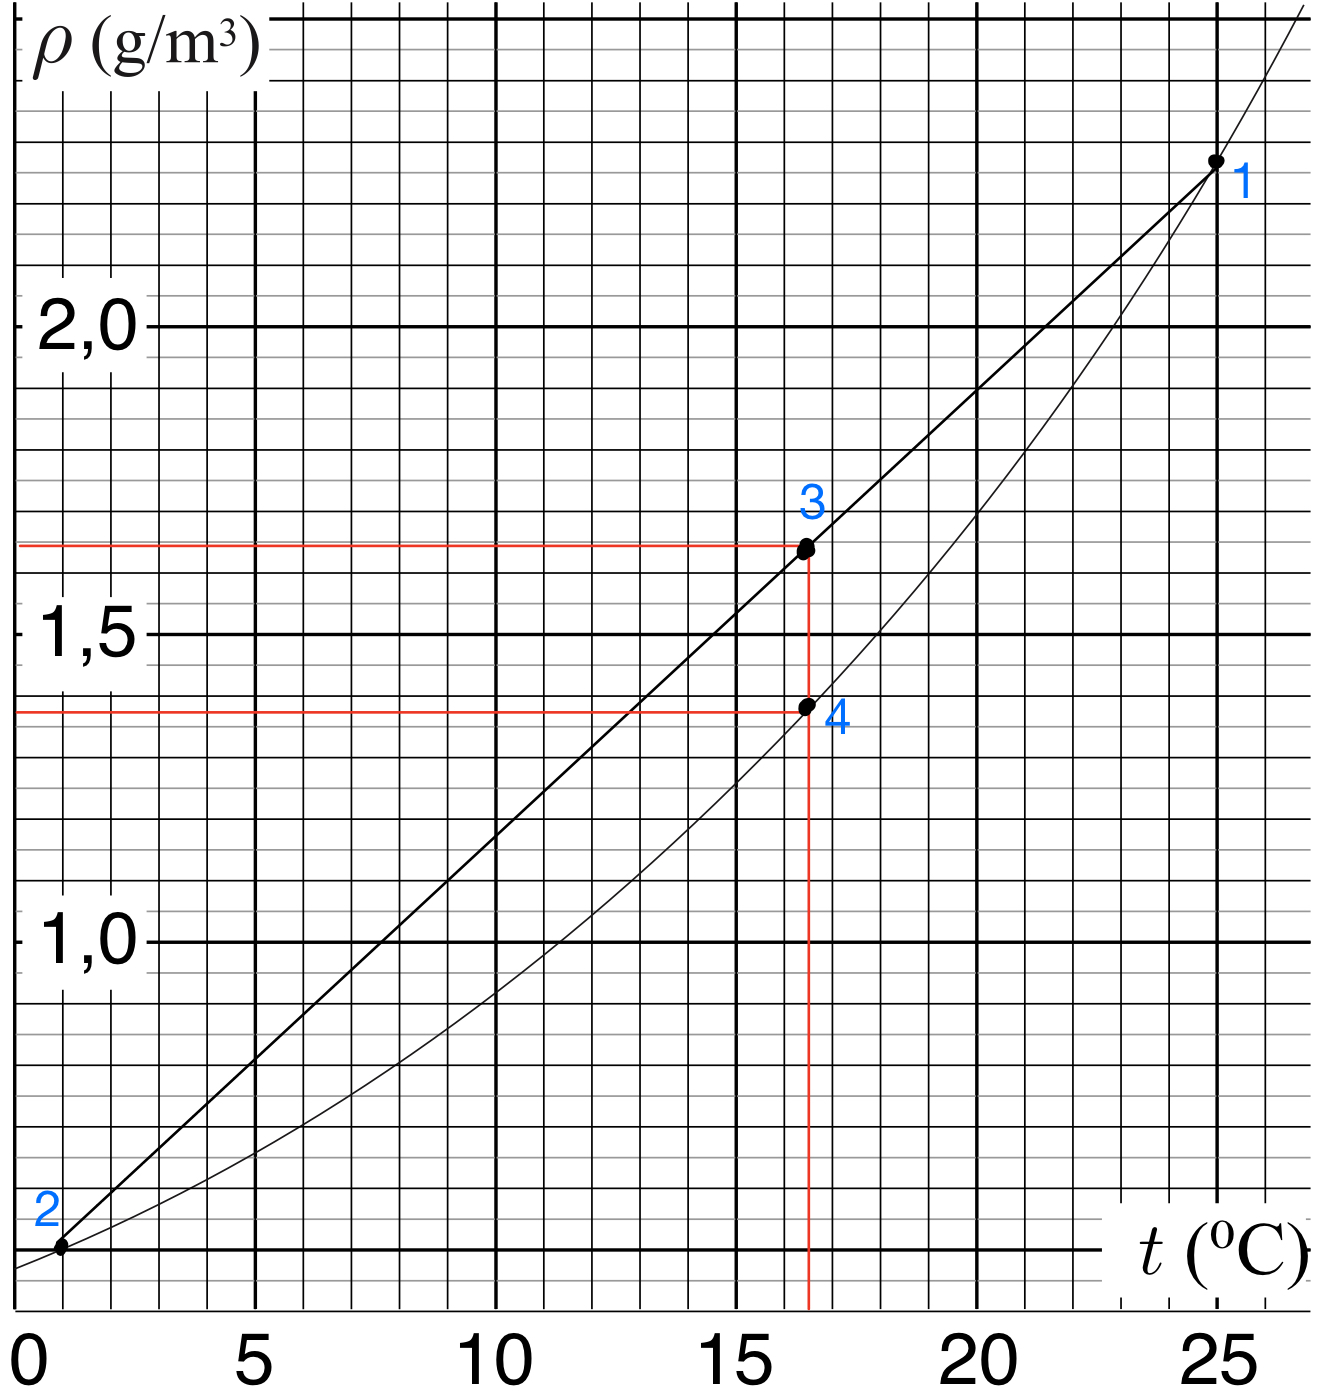
\includegraphics[width=10cm]{B89B8B17-45E5-4913-9313-C1B06F8B168D.jpeg}
\end{center}
\vspace{3mm}

\noindent \textbf{(d)} The mass will have to undergo a small temperature change to condensate. This means that it will have to transfer heat to its surroundings and with that information, we can attempt to balance the heat going out into the system and the heat going into the system. The heat going out of the system moves to the surrounding and will go to the outside air that has a given density $\rho_0$. With a temperature change denoted by $\Delta t$, we write $Q_{\text{out}} = mc\Delta T = \rho_0 V c\Delta t$. The heat going into the surroundings changes the temperature of the mixed air. If $t^{\prime} = 16.5^{\circ}\;\mathrm{C}$ is the initial temperature of the mixed air, we write $Q = q(\rho_{\text{v}} (t^{\prime} - \rho_{\text{vs}} (t^{\prime} + \Delta t))$. We conserve heat to get the equation
\[\rho_0 c\Delta t = q (\rho_{\text{v}} (t^{\prime} - \rho_{\text{vs}} (t^{\prime} + \Delta t)).\]We then find by rearranging variables that
\[\rho_{\text{vs}} (t^{\prime} + \Delta t) = \rho_v (t^{\prime}) - \frac{\rho_0 c_p \Delta t}{q}.\]Let us denote $T = t^{\prime} + \Delta t$. This means that $\Delta t = T - t^{\prime}$. Our equation then looks like
\[\rho_{\text{vs}} (T) = 1.65 - 0.47 (T - 16.5).\]This is an equation of a line, and the intersection of this line with the graph of the saturated vapor density gives us the new condensated mass. As shown in the picture below, we have our new point 5 to be the density of the new mass. Remember that we have to find the new mass of the condensated mass which will be given by $m = \Delta \rho (V_1 + V_2)$. We see that $\Delta \rho \approx 0.25\;\mathrm{g/m^3}$ from the graph so $m \approx 7.5\;\mathrm{g}$.
\begin{center}
    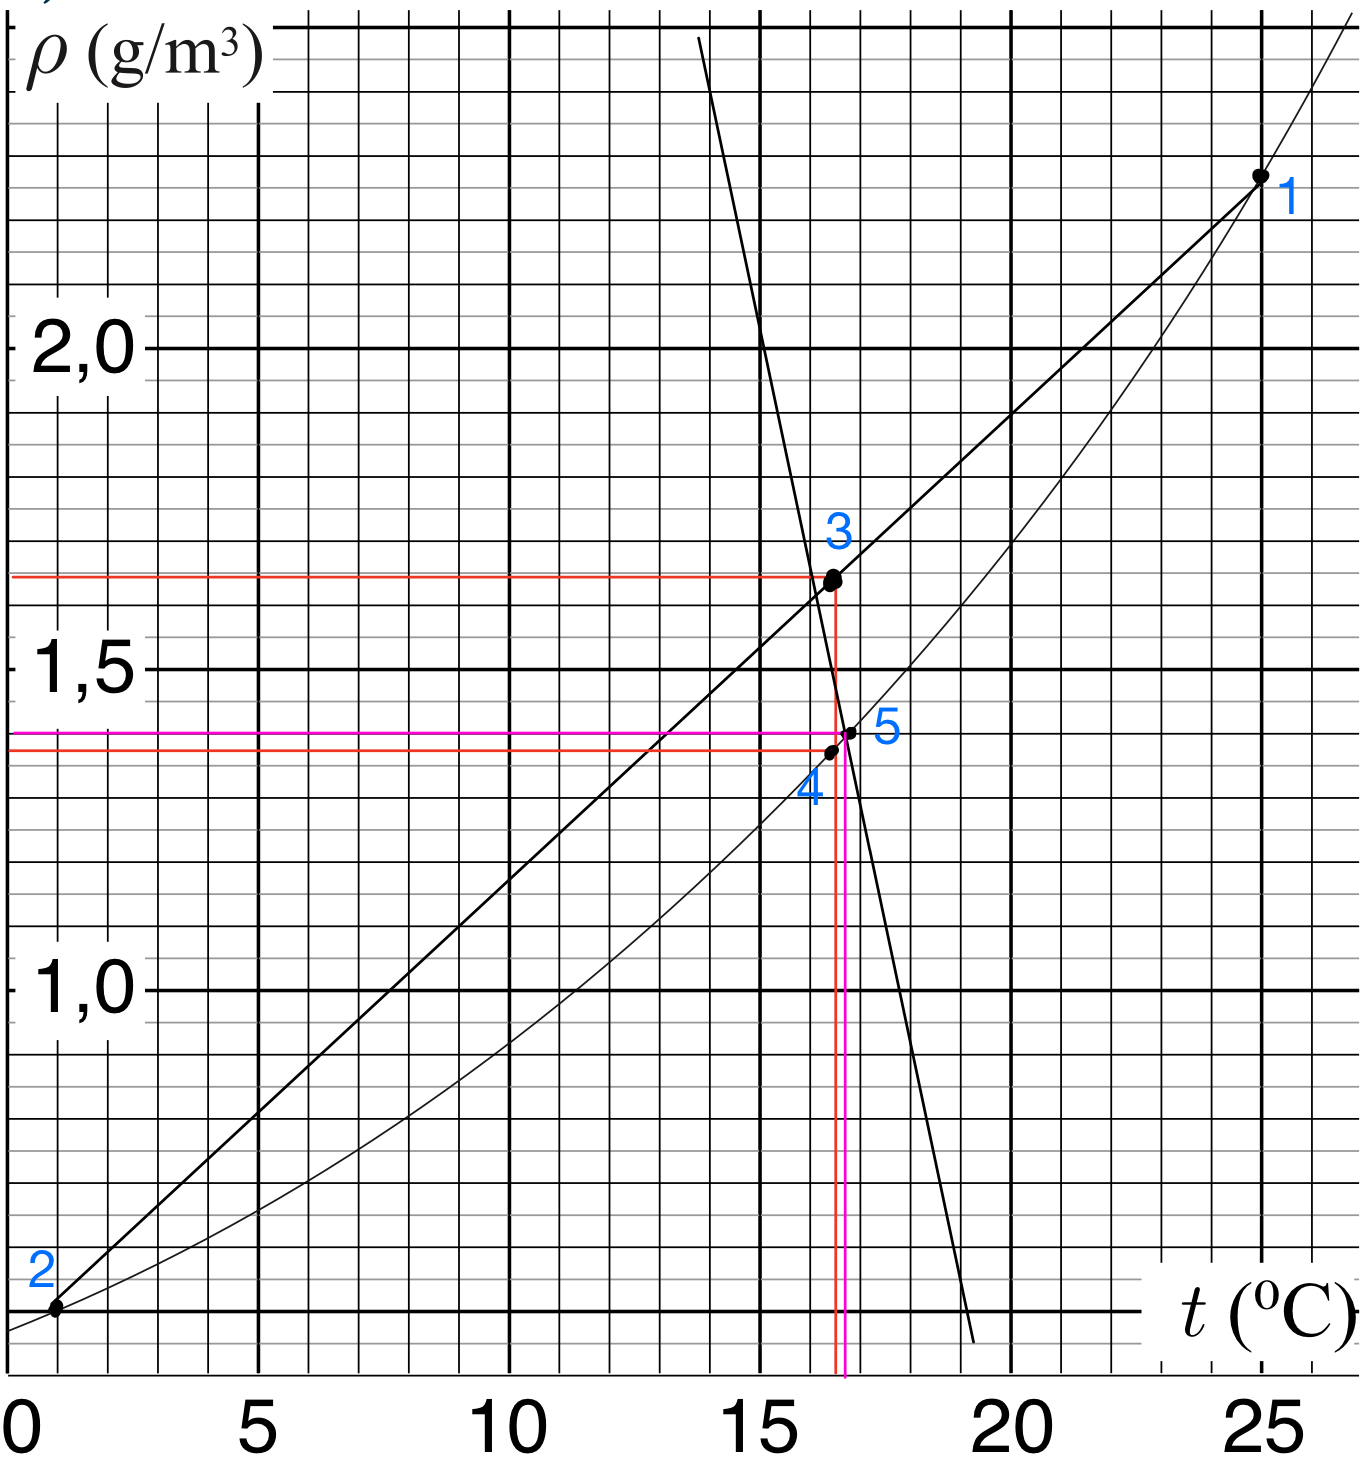
\includegraphics[width=10cm]{9B2F586B-C0CE-40D7-8A66-83E5A94057A5.jpeg}
\end{center}
\end{solution}